\documentclass{beamer}

\usetheme{Boadilla}
\beamertemplatenavigationsymbolsempty

\usepackage{graphicx}
\usepackage{subcaption}
\usepackage{amsthm}
\usepackage{amsmath}
\usepackage{listings}

\title{docmgr Result}
\subtitle{Word index manager for documents}
\author[Facundo E. \and Iñaki R.]{Facundo Escobar \and Iñaki Rodriguez}
\institute[UnCuyo]{Universidad Nacional de Cuyo}
\date{\today}

\newtheorem{blkquote}{Quote}

\begin{document}

\begin{frame}
  \titlepage
\end{frame}

\begin{frame}[c]
  \frametitle{Command line syntax}
  \centering
  \texttt{docmgr [options] [file1 file2 ...]}
\end{frame}

\begin{frame}
  \frametitle{Data structure employed}
  \begin{figure}
    \includegraphics[width=0.3\linewidth]{structure.png}
    \caption{Representation of the project data structure.}
    \label{fig:structure1}
  \end{figure}
\end{frame}

\begin{frame}
  \frametitle{Found problems}
  \begin{enumerate}
    \item Using Git version control.
  \end{enumerate}
  \begin{figure}[h!]
    \includegraphics[width=0.3\linewidth]{Git-Logo-2Color.png}
    \caption{\texttt{git} may be a little difficult for the beginner.}
    \label{fig:git3}
  \end{figure}
\end{frame}

\begin{frame}
  \frametitle{Found problems}
  \begin{enumerate}
    \setcounter{enumi}{1}
    \item Pickle serialization and deserialization.
  \end{enumerate}
  \begin{blkquote}
    \texttt{pickle} is a pickle.
  \end{blkquote}
\end{frame}

\begin{frame}[fragile]
  \frametitle{Found problems}
  \begin{enumerate}
    \setcounter{enumi}{2}
    \item Insertion in the Trie.
  \end{enumerate}
  \begin{lstlisting}[
    frame=single,
    language=Python,
    keywordstyle=\color{orange},
    keywordstyle={[2]\color{purple2}},
    stringstyle=\color{green2},
    commentstyle=\color{gray},
  ]
  insert(trie, key)           # vs
  insert(trie, key, value)
  \end{lstlisting}
\end{frame}

\begin{frame}
  \frametitle{Found problems}
  \begin{enumerate}
    \setcounter{enumi}{3}
    \item Resizing the hashmap.
  \end{enumerate}
  \begin{figure}
    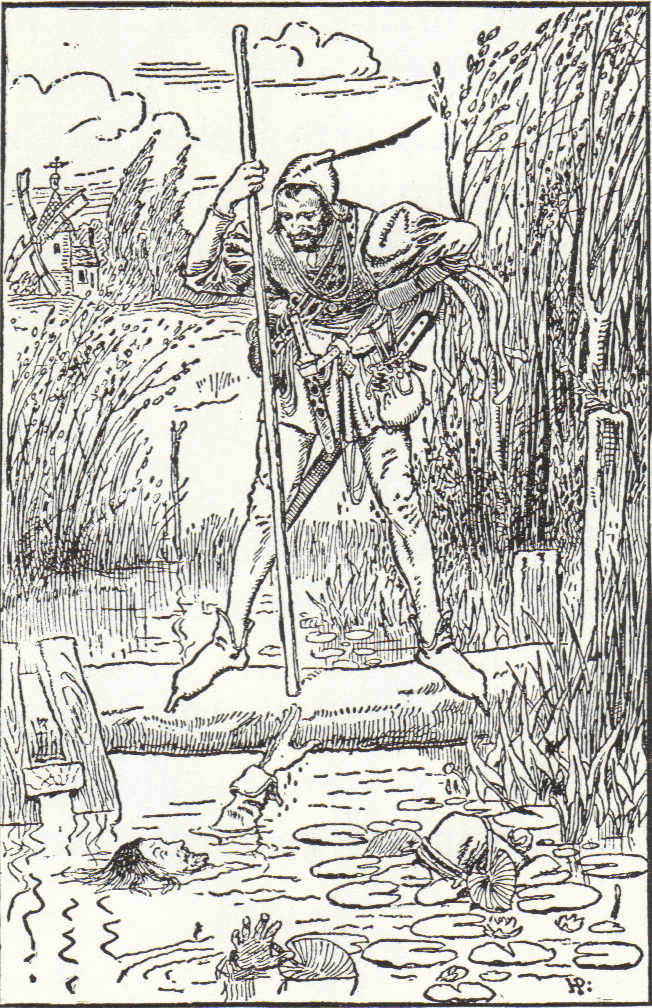
\includegraphics[width=0.3\linewidth]{Robin-hood-at-the-lake-01.png}
    \caption{\textit{Robin Hood} hashmaps resizing tripped and fell.}
    \label{fig:robinhood2}
  \end{figure}
\end{frame}

\begin{frame}
  \frametitle{Analyzed complexities}
  Time complexity of \texttt{create()}.
  \begin{align*}
     & \text{\texttt{hash\_search()}:} & O(d) \And \Omega(1)                                       \\
     & \text{\texttt{hash\_insert()}:} & O(d) \And \Omega(1)                                       \\
     & \text{\texttt{insert()}:}       & O(\left\vert \Sigma \right\vert * w)                      \\
     & \text{\texttt{index\_words()}:} & O(t + qw * (\left\vert \Sigma \right\vert * w + d))       \\
     & \text{\texttt{index\_docs()}:}  & O(d * (t + qw * (\left\vert \Sigma \right\vert * w + d))) \\
     & \text{\texttt{create()}:}       & O(d * (t + qw * (\left\vert \Sigma \right\vert * w + d)))
  \end{align*}
\end{frame}

\begin{frame}
  \frametitle{Analyzed complexities}
  Time complexity of \texttt{search()}.
  \begin{align*}
     & \text{\texttt{merge\_sort()}:} & O(n \log{n}) \\
     & \text{\texttt{print\_hash()}:} & O(n)         \\
     & \text{\texttt{search()}:}      & O(n)
  \end{align*}
\end{frame}

\begin{frame}
  \frametitle{Analyzed complexities}
  Space complexity of the data structure.
  \begin{align*}
     & \text{\texttt{HashTable}:} & O(d)           \\
     & \text{\texttt{Trie}:}      & O((k + d) * w)
  \end{align*}
\end{frame}

\end{document}
